
Para que seja possível controlar os dois rotores por meio de controladores PID ou por realimentação de estados, é necessário desacoplar os sistemas. Isso é obtido reduzindo-se a influência que as FTs do \textit{cross-pitch} e \textit{cross-yaw} desempenham sobre o comportamento resultante dos ângulos de arfagem e guinada. Assim, esta seção busca descrever o projeto de desacoplamento adotado, bem como sua validação, em malha aberta, por meio de simulação.

\subsection{\textbf{Projeto dos Desacopladores}}

De acordo com \cite{seborg2010process}, o desacoplamento dos sistemas pode ser realizado projetando-se FTs $T_{12}(s)$ e $T_{21}(s)$ de forma que, quando conectadas ao sistema, como mostrado na Figura \ref{fig:ProjetoDesacopla}, sejam cancelados ou atenuados os efeitos de $G_{cp}(s)$ e de $G_{cy}(s)$.

\begin{figure}[H]
    \centering
    \includegraphics[width=0.48\textwidth]{figures/Desacoplamento/Desacoplamento.pdf}
    \caption{Diagrama de blocos do sistema MIMO com desacopladores.}
    \label{fig:ProjetoDesacopla}
\end{figure}

Assumindo-se inicialmente, que $U_{22} = 0$ e que $U_{11} \neq 0$, tem-se que
\begin{equation}\label{eq:T21}
    U_{21} = T_{21} U_{11}
\end{equation}
\noindent para desacoplar $G_{21}$, deve-se obter
\begin{equation}\label{eq:DesG21}
    U_{11} G_{21} + U_{21} G_{22} = 0
\end{equation}
\noindent substituindo \eqref{eq:T21} em \eqref{eq:DesG21} e isolando-se $T_{21}$:
\begin{equation}\label{eq:DesT21}
    T_{21} = - \frac{G_{21}}{G_{22}}
\end{equation}
Substituindo as FTs \eqref{eq:FTModeloIDCrossPitch} $G_{21}$ e \eqref{eq:FTModeloIDYaw} $G_{22}$ em \eqref{eq:DesT21FT}, obtém-se
\begin{equation}\label{eq:DesT21FT}
    T_{21} = - \frac{0.024987 (s+0.5231) (s^2 + 0.2437s + 4.123)}{s^2 + 0.6339s + 4.262}
\end{equation}
Aplicando-se o mesmo processo, agora para $U_{11} = 0$ e $U_{22} \neq 0$, é possível obter uma expressão para $T_{12}$ que desacopla $G_{12}$:
\begin{equation}\label{eq:T12}
    U_{12} = T_{12} U_{22}
\end{equation}
\begin{equation}\label{eq:DesG12}
    U_{22} G_{12} + U_{12} G_{11} = 0
\end{equation}
\noindent substituindo \eqref{eq:T12} em \eqref{eq:DesG12} e isolando-se $T_{12}$:
\begin{equation}\label{eq:DesT12}
    T_{12} = - \frac{G_{12}}{G_{11}}
\end{equation}
Substituindo as FTs \eqref{eq:FTModeloIDCrossYaw} $G_{12}$ e \eqref{eq:FTModeloIDPitch} $G_{11}$ em \eqref{eq:DesT12FT}, obtém-se
\begin{equation}\label{eq:DesT12FT}
    T_{12} = - \frac{0.8299 (s+0.06236) (s^2 + 0.3948s + 0.2209)}{s^2 + 0.2574s + 0.1437}
\end{equation}
Das equações \eqref{eq:DesT21FT} e \eqref{eq:DesT12FT} para $T_{12}$ e $T_{21}$, vê-se que foram obtidas equações não realizáveis na prática. Com base nisso, buscou-se aproximar essas equações desacoplamento apenas pelo seus ganhos estáticos. O que é equivalente a desacoplar os sistemas em regime permanente \cite{seborg2010process}.
\begin{equation}\label{eq:T21Gain}
    T_{{21}_{k}} = -0.024987
\end{equation}
\begin{equation}\label{eq:T12Gain}
    T_{{12}_{k}} = -0.829900
\end{equation}
Após ajustes desses ganhos com objetivo de melhorar o desacoplamento, obteve-se
\begin{equation}\label{eq:T21GainFinal}
    T_{{21}_{k}} = -0.05
\end{equation}
\begin{equation}\label{eq:T12GainFinal}
    T_{{12}_{k}} = -0.07
\end{equation}
Esses valores foram utilizados nas simulações de validação do desacoplamento, cujos resultados são mostrados na próxima seção.

\subsection{\textbf{Validação do Desacoplamento}}

A validação do desacoplamento projetado foi realizada por meio da aplicação de dois sinais de entrada: um do tipo pulso e uma senoide. Foram analisados os sinais do \textit{pitch} e \textit{yaw}, \textit{cross-pitch} e \textit{cross-yaw}, assim como da soma de \textit{cross-yaw} com \textit{pitch} e \textit{cross-pitch} com o \textit{yaw}. A ideia foi a de mostrar que a influência das FTs do \textit{cross-pitch} e \textit{cross-yaw} foram reduzidas após a inserção dos desacopladores, fazendo com que o sinal proveniente da soma e o sinal direto ficassem mais próximos.

%%%%%%%%%%%%%%%%%%%%%%%%%%%%%%%%%%%%%%%% PITCH

Na Figuras \ref{fig:PitchAcopladoPulso}, \ref{fig:PitchDesacopladoPulso}, \ref{fig:PitchAcopladoSenoide} e \ref{fig:PitchDesacopladoSenoide} são mostrados os resultados da aplicação dos sinais mencionados para o \textit{pitch}, mostrando o comportamento dos sinais antes (acoplados) e após (desacoplados).

\begin{figure}[H]
    \centering
    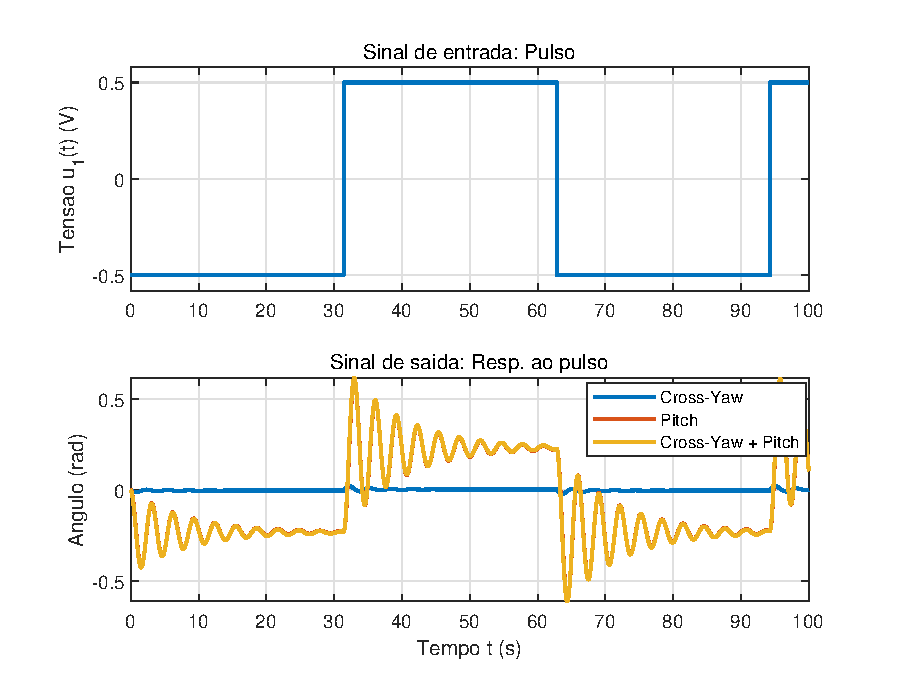
\includegraphics[width=0.48\textwidth]{figures/Desacoplamento/Pitch_Acoplado_Pulso.eps}
    \caption{Ângulo do \textit{pitch}: Acoplado.}
    \label{fig:PitchAcopladoPulso}
\end{figure}

\begin{figure}[H]
    \centering
    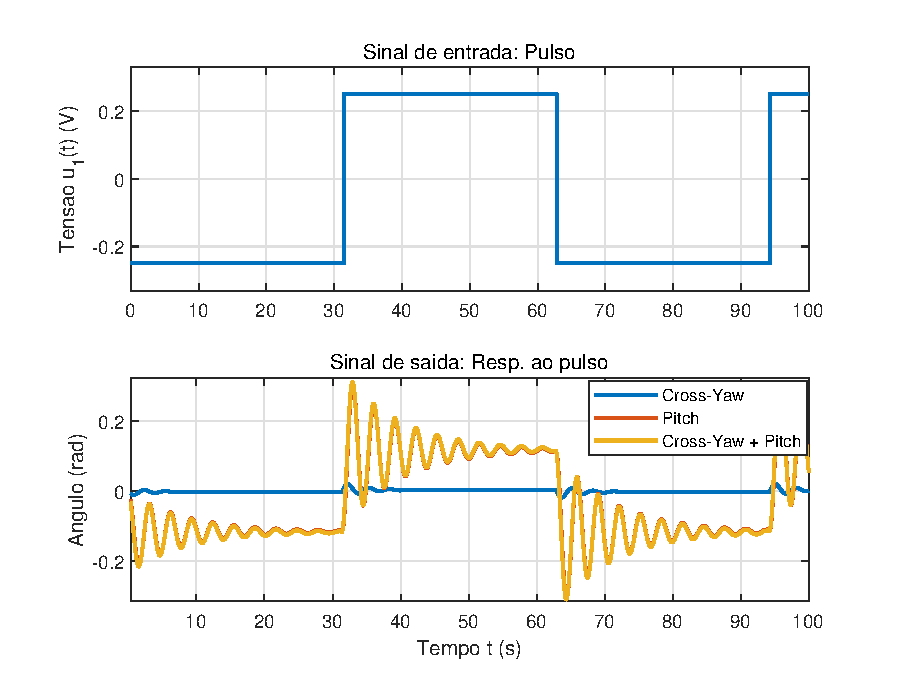
\includegraphics[width=0.48\textwidth]{figures/Desacoplamento/Pitch_Desacoplado_Pulso.eps}
    \caption{Ângulo do \textit{pitch}: Desacoplado.}
    \label{fig:PitchDesacopladoPulso}
\end{figure}

\begin{figure}[H]
    \centering
    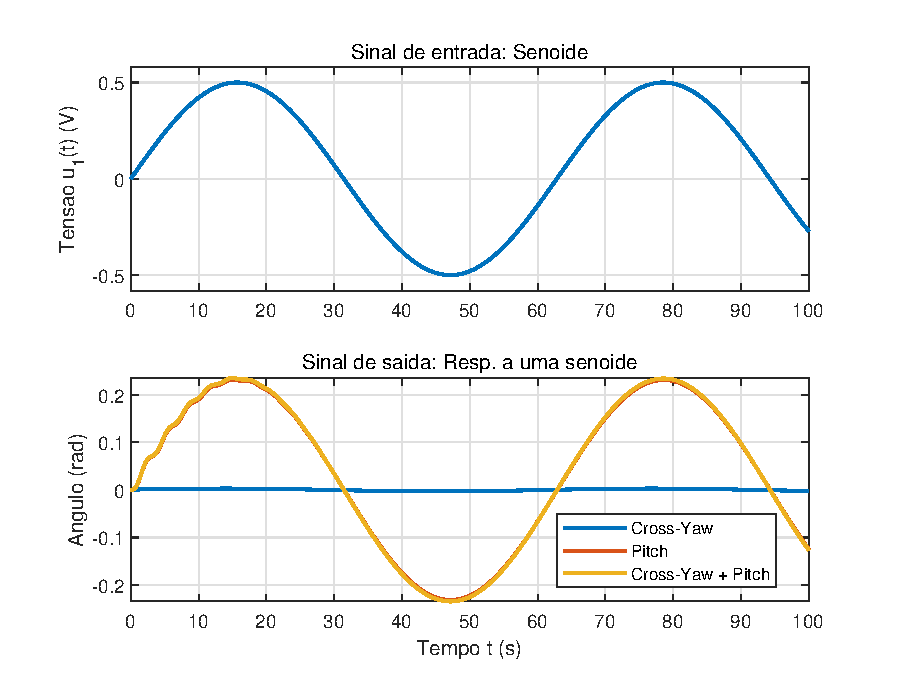
\includegraphics[width=0.48\textwidth]{figures/Desacoplamento/Pitch_Acoplado_Senoide.eps}
    \caption{Ângulo do \textit{pitch}: Acoplado.}
    \label{fig:PitchAcopladoSenoide}
\end{figure}

\begin{figure}[H]
    \centering
    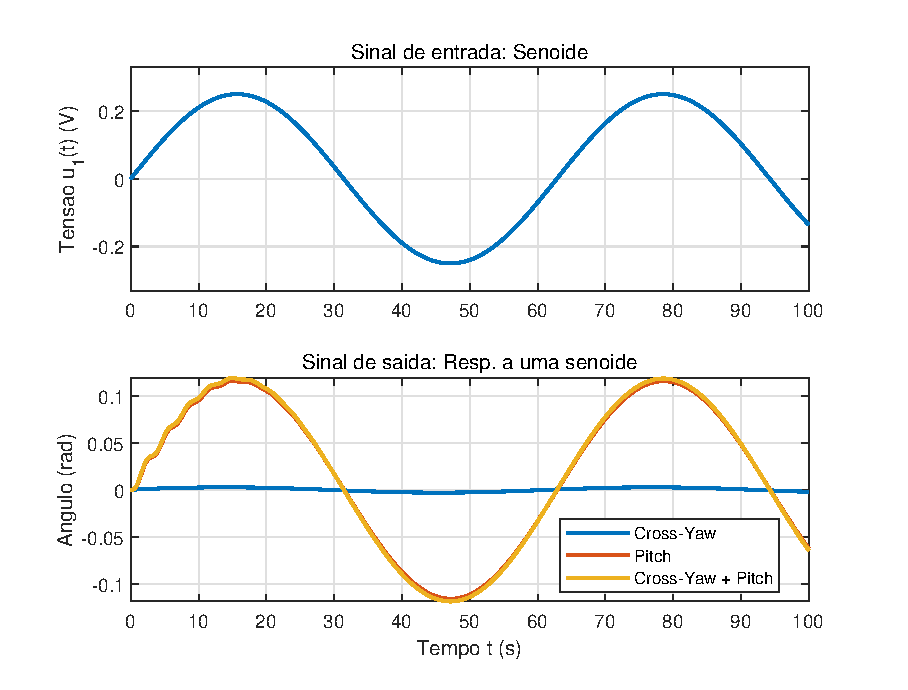
\includegraphics[width=0.48\textwidth]{figures/Desacoplamento/Pitch_Desacoplado_Senoide.eps}
    \caption{Ângulo do \textit{pitch}: Desacoplado.}
    \label{fig:PitchDesacopladoSenoide}
\end{figure}

Para os dois tipos de sinais aplicados, vê-se que o comportamento do ângulo do \textit{pitch} não melhorou de forma perceptiva. Isso se deve ao fato de que a influência da FT do \textit{cross-yaw} ser muito pequena, como pode ser observado nas Figuras \ref{fig:IdentificacaoCrossYawInicial} e \ref{fig:IdentificacaoCrossYawFinal}, obtidas no processo de identificação do modelo, nas quais o ganho da FT é da ordem de $\SI{1e-3}{}$.

%%%%%%%%%%%%%%%%%%%%%%%%%%%%%%%%%%%%%%%% YAW

Na Figuras \ref{fig:YawAcopladoPulso}, \ref{fig:YawDesacopladoPulso}, \ref{fig:YawAcopladoSenoide} e \ref{fig:YawDesacopladoSenoide} são mostrados os resultados obtidos antes e após o desacoplamento dos ângulos.

\begin{figure}[H]
    \centering
    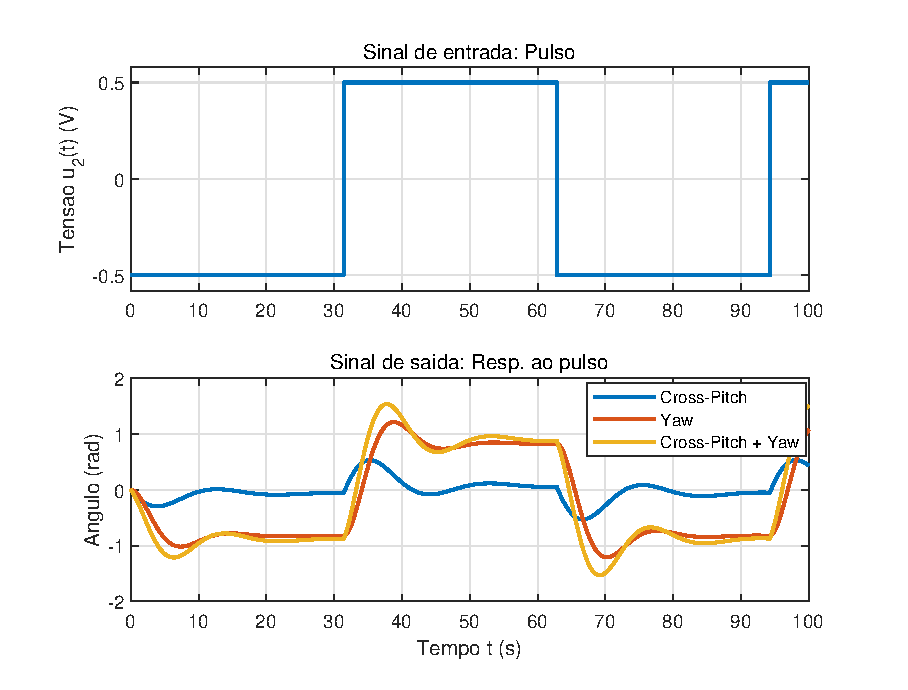
\includegraphics[width=0.48\textwidth]{figures/Desacoplamento/Yaw_Acoplado_Pulso.eps}
    \caption{Ângulo do \textit{yaw}: Acoplado.}
    \label{fig:YawAcopladoPulso}
\end{figure}

\begin{figure}[H]
    \centering
    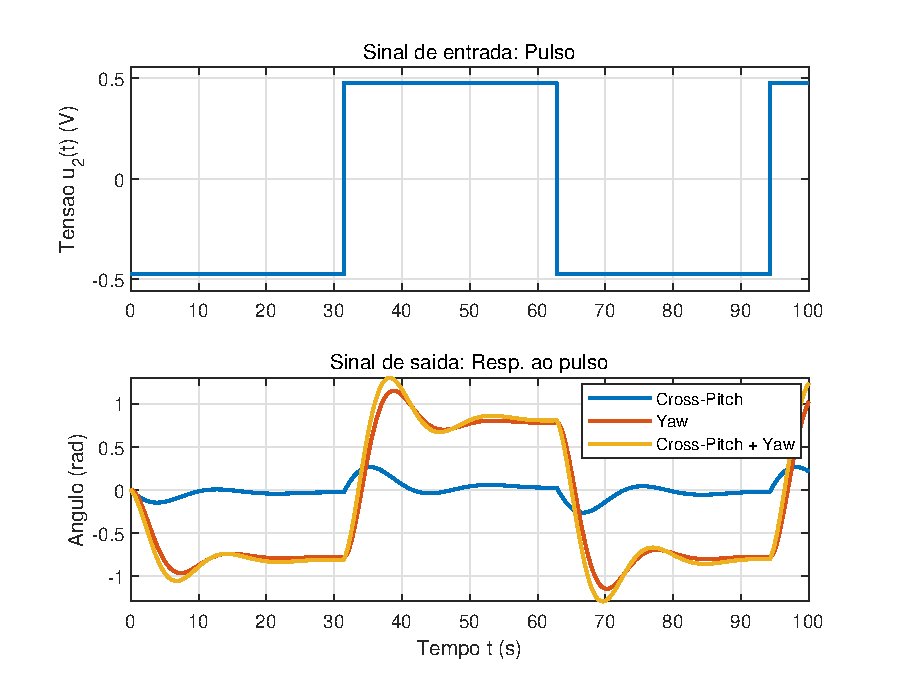
\includegraphics[width=0.48\textwidth]{figures/Desacoplamento/Yaw_Desacoplado_Pulso.eps}
    \caption{Ângulo do \textit{yaw}: Desacoplado.}
    \label{fig:YawDesacopladoPulso}
\end{figure}


\begin{figure}[H]
    \centering
    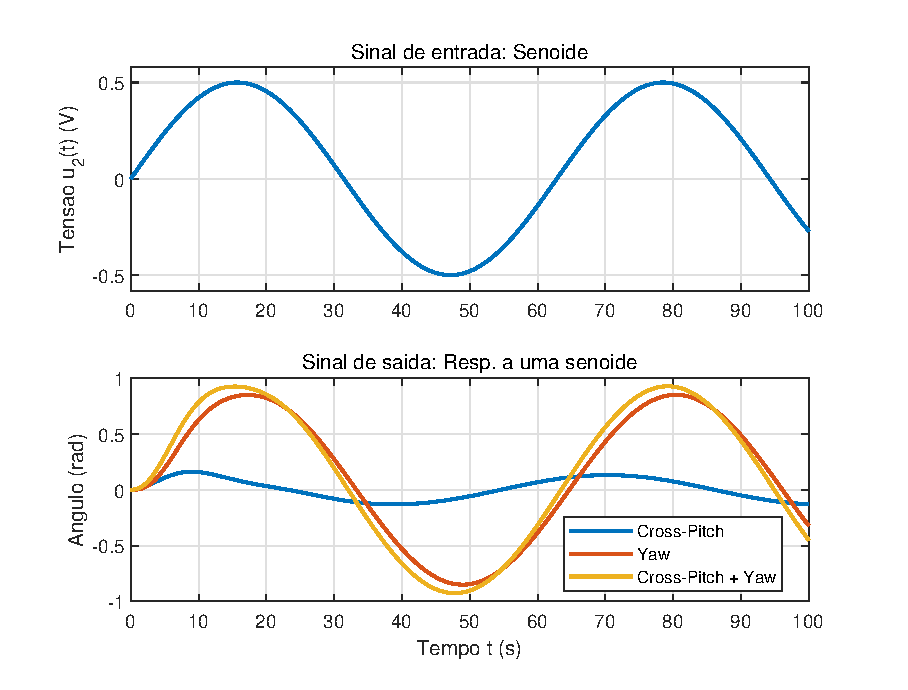
\includegraphics[width=0.48\textwidth]{figures/Desacoplamento/Yaw_Acoplado_Senoide.eps}
    \caption{Ângulo do \textit{yaw}: Acoplado.}
    \label{fig:YawAcopladoSenoide}
\end{figure}

\begin{figure}[H]
    \centering
    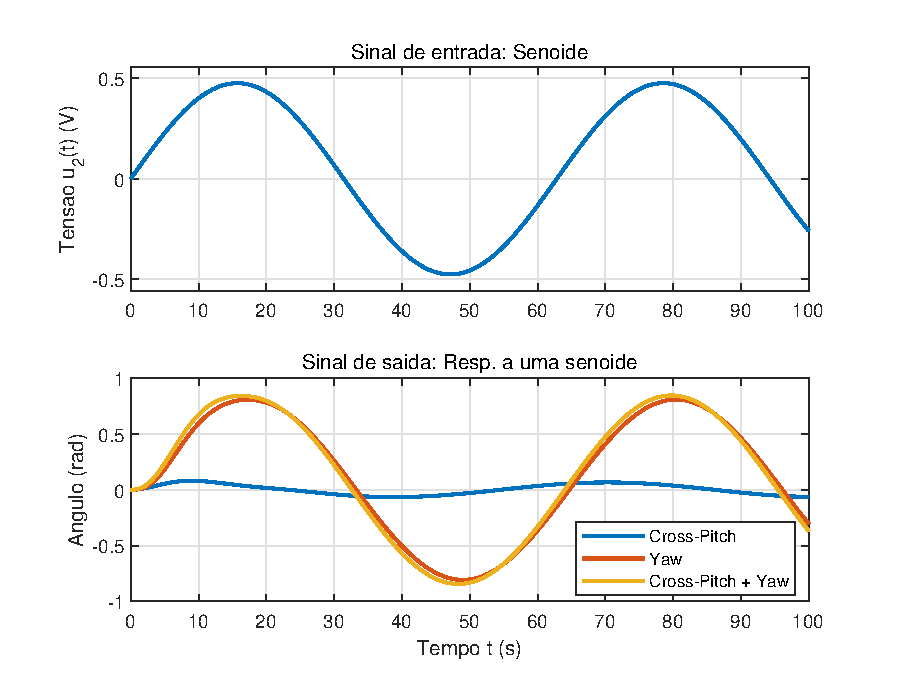
\includegraphics[width=0.48\textwidth]{figures/Desacoplamento/Yaw_Desacoplado_Senoide.eps}
    \caption{Ângulo do \textit{yaw}: Desacoplado.}
    \label{fig:YawDesacopladoSenoide}
\end{figure}

Ao contrário do observado para o \textit{pitch}, vê-se que o desacoplamento foi capaz de reduzir a influência do \textit{cross-pitch} à aproximadamente a metade, com seu valor máximo de pico reduzindo de $\approx 0.5$ para $\approx 0.25$ (Figuras \ref{fig:YawAcopladoPulso} e \ref{fig:YawDesacopladoPulso}). A redução do acoplamento é percebida também na aplicação do sinal senoidal.